\section{198 --- House Robber (LeetCode)}

\subsection*{Código}
\lstinputlisting{198_HouseRobber.java}

\subsection*{Comprovante de aceite}
\begin{center}
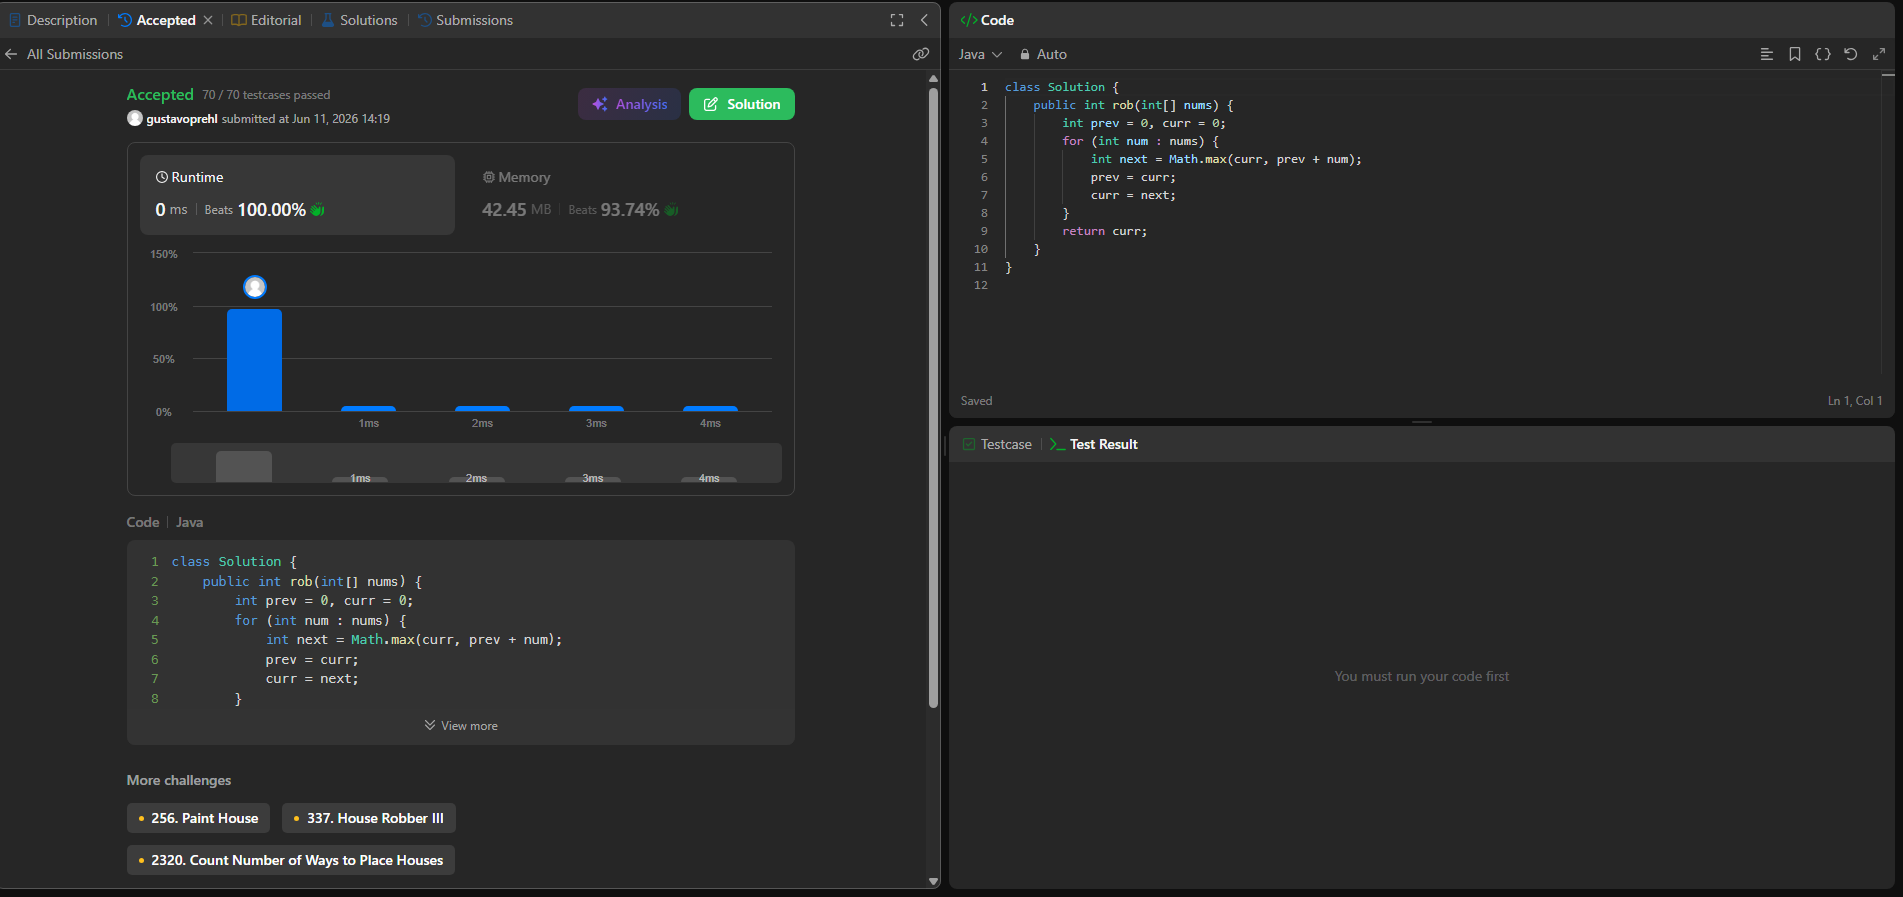
\includegraphics[width=0.85\textwidth]{Accepts/198_HouseRobber_Submit.png}\\
\end{center}

\subsection*{Justificativa}

\textbf{Estratégia:} programação dinâmica (\emph{bottom-up}, com otimização
de espaço).

\textbf{Subestrutura ótima:} seja $dp[i]$ o valor máximo que se pode roubar
considerando apenas as primeiras $i$ casas. Para a casa $i$, há exatamente
duas opções:
\begin{itemize}
    \item \textbf{não roubar a casa $i$}: o melhor valor é $dp[i-1]$;
    \item \textbf{roubar a casa $i$}: como a casa $i-1$ não pode ter sido
    roubada, o melhor valor é $dp[i-2] + nums[i]$.
\end{itemize}

Logo, a recorrência é:
\[
dp[i] = \max\big(dp[i-1],\; dp[i-2] + nums[i]\big)
\]

A solução ótima global é construída a partir das soluções ótimas de
subproblemas menores (prefixos do array), o que caracteriza a propriedade de
\textbf{subestrutura ótima}.

\textbf{Subproblemas sobrepostos:} $dp[i-1]$ e $dp[i-2]$ são reutilizados
repetidamente no cálculo de $dp[i]$, $dp[i+1]$, etc. Em vez de recalcular
esses valores recursivamente (o que levaria a complexidade exponencial), a
abordagem \emph{bottom-up} resolve cada subproblema uma única vez, em ordem
crescente de $i$, armazenando o resultado.

\textbf{Otimização de espaço:} como $dp[i]$ depende apenas dos dois valores
anteriores, não é necessário manter o vetor $dp$ inteiro --- basta guardar
\texttt{prev} ($= dp[i-2]$) e \texttt{curr} ($= dp[i-1]$), atualizando-os a
cada iteração.

\textbf{Complexidade:}
\begin{itemize}
    \item Tempo: $O(n)$, uma única passagem pelo array.
    \item Espaço: $O(1)$, apenas duas variáveis auxiliares.
\end{itemize}

\textbf{Tópico do curso:} \emph{Programação Dinâmica} [CLRS09, cap. 15] ---
identificação de subestrutura ótima e subproblemas sobrepostos, com
formulação da recorrência \emph{bottom-up} e otimização do espaço de
armazenamento.
